Теперь рассмотрим дисперсионные соотношения. Начнём c LE-волн. Поперечные
волновые числа получаются из решения систем
\[
    \left\{
        \begin{array}{l}
            u_2^2 - u_1^2 = \omega^2(\eps_2\mu_2 - \eps_1\mu_1), \\
            \frac{\mu_1\tg u_1 (a-c)}{u_1} + \frac{\mu_2\tg u_2 c}{u_2}
            = 0
        \end{array}
    \right.
\]
для быстрых волн и
\[
    \left\{
        \begin{array}{l}
            u_2^2 + u_1^2 = \omega^2(\eps_2\mu_2 - \eps_1\mu_1), \\
            \frac{\mu_1\th u_1 (a-c)}{u_1} + \frac{\mu_2\tg u_2 c}{u_2} = 0
        \end{array}
    \right.
\]
для поверхностной волны. Аналитически они не решаются, поэтому представим
результаты численного решения графически. Для отображения обоих классов волн на
одном графике для поверхностной волны будем считать \( u_1^2 < 0 \). Тогда
первые уравнение систем изобразятся прямой, положение которой определяется
частотой, а вторые -- семейством непрерывных кривых. Полученная картина
представлена на рисунке~\ref{fig:le_dispersion}.

\begin{figure}[h]
    \center
    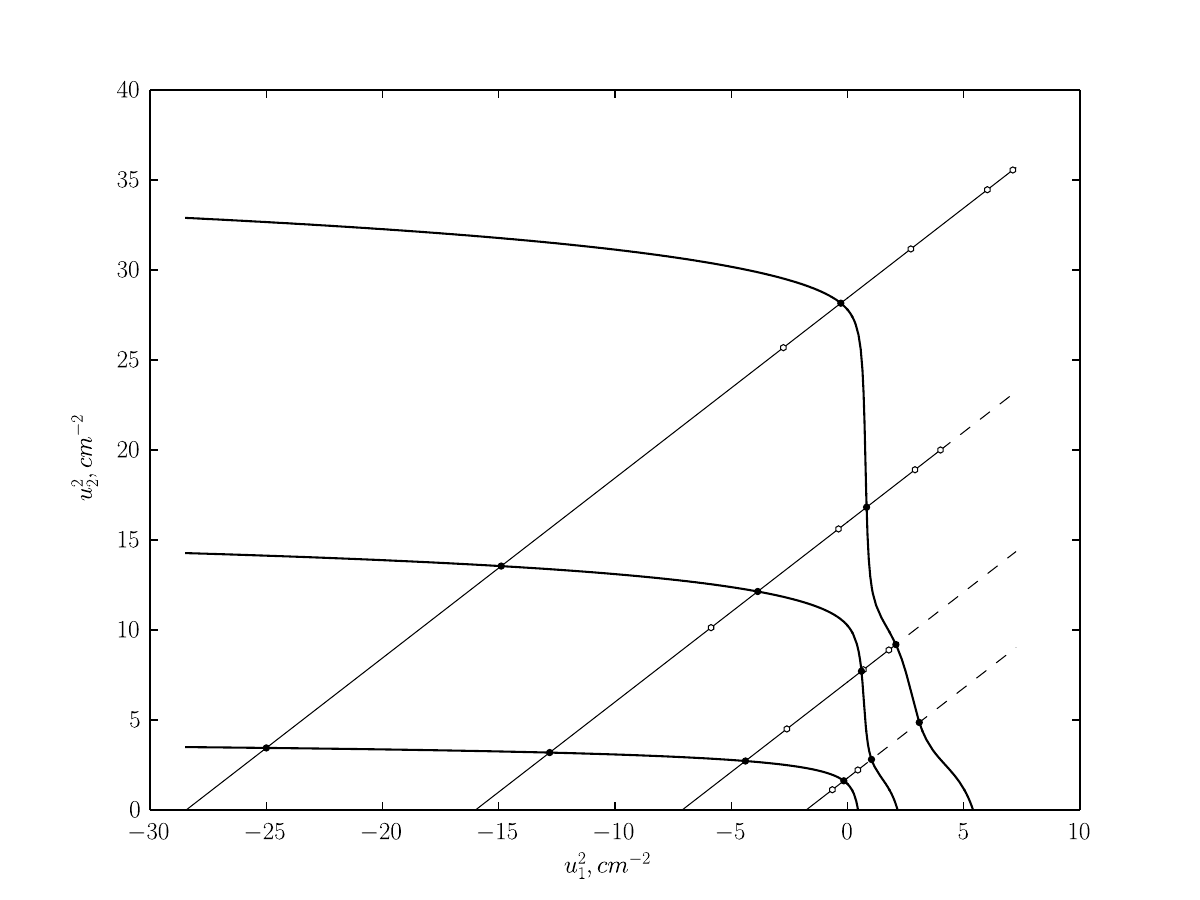
\includegraphics[width=.7\textwidth]{dispersion/le.png}
    \caption{К определению поперечных волновых чисел для LE-волн}
    \label{fig:le_dispersion}
\end{figure}


Совершенно аналогично поступим с LM-волнами. Для них системы имеют вид
\[
    \left\{
        \begin{array}{l}
            u_2^2 - u_1^2 = \omega^2(\eps_2\mu_2 - \eps_1\mu_1), \\
            \frac{u_1\tg u_1 (a-c)}{\eps_1} + \frac{u_2\tg u_2 c}{\eps_2}
            = 0
        \end{array}
    \right.
\]
для быстрых волн и
\[
    \left\{
        \begin{array}{l}
            u_2^2 + u_1^2 = \omega^2(\eps_2\mu_2 - \eps_1\mu_1), \\
            -\frac{u_1\th u_1 (a-c)}{\eps_1} + \frac{u_2\tg u_2 c}{\eps_2} = 0
        \end{array}
    \right.
\]
для поверхностной. Здесь график будет иметь вид, представленный на
рисунке~\ref{fig:lm_dispersion}.

\begin{figure}[h]
    \center
    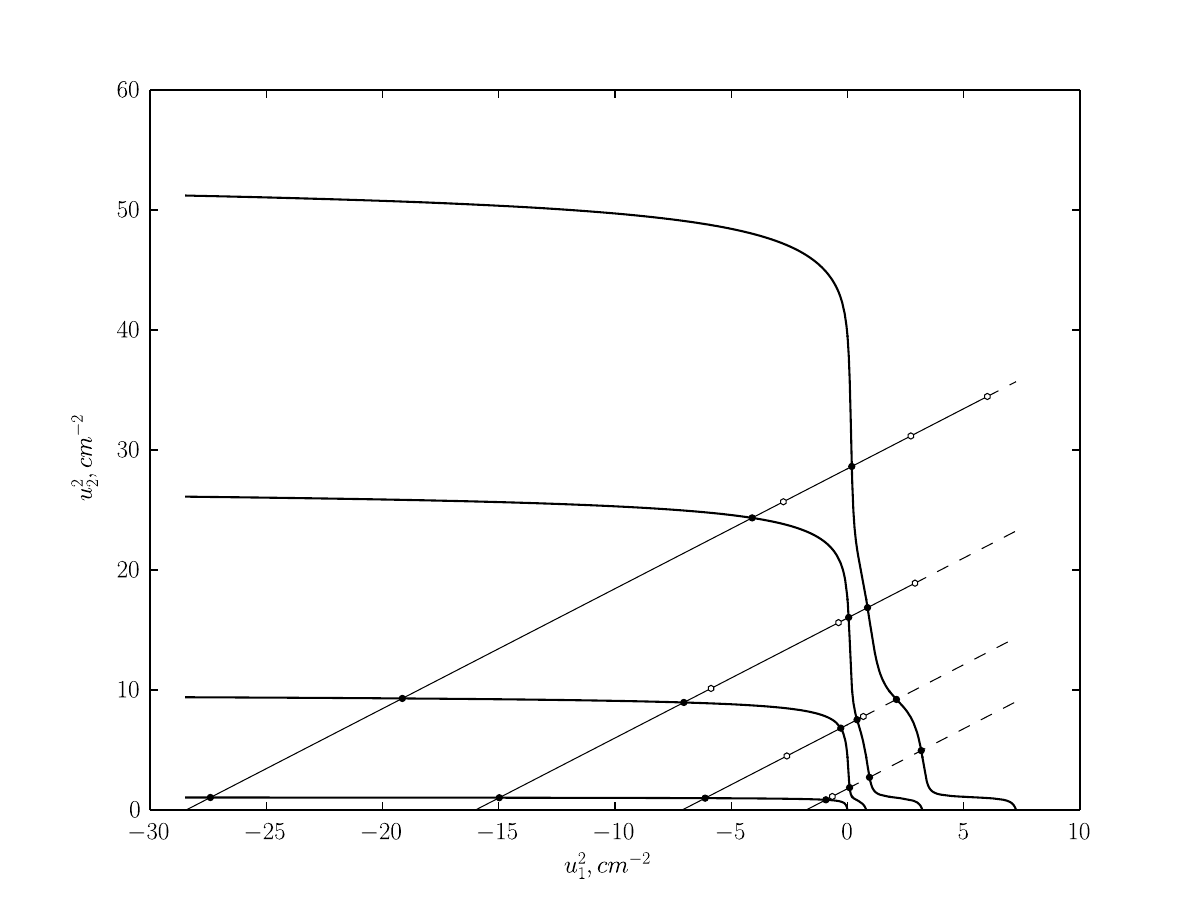
\includegraphics[width=.7\textwidth]{dispersion/lm.png}
    \caption{К определению поперечных волновых чисел для LM-волн}
    \label{fig:lm_dispersion}
\end{figure}

По известным поперечным волновым числам легко определяется продольное:
\[
    h = \sqrt{\beta_2^2 - u_2^2 - \left(\frac{\pi n}{b}\right)^2}.
\]
Таким образом, можно получить закон дисперсии \( h(\omega) \), представленный на
рисунке~\ref{fig:dispersion}. Здесь штриховой линией отмечены поверхностные
волны, а сплошной -- быстрые.

\begin{figure}[H]
    \center
    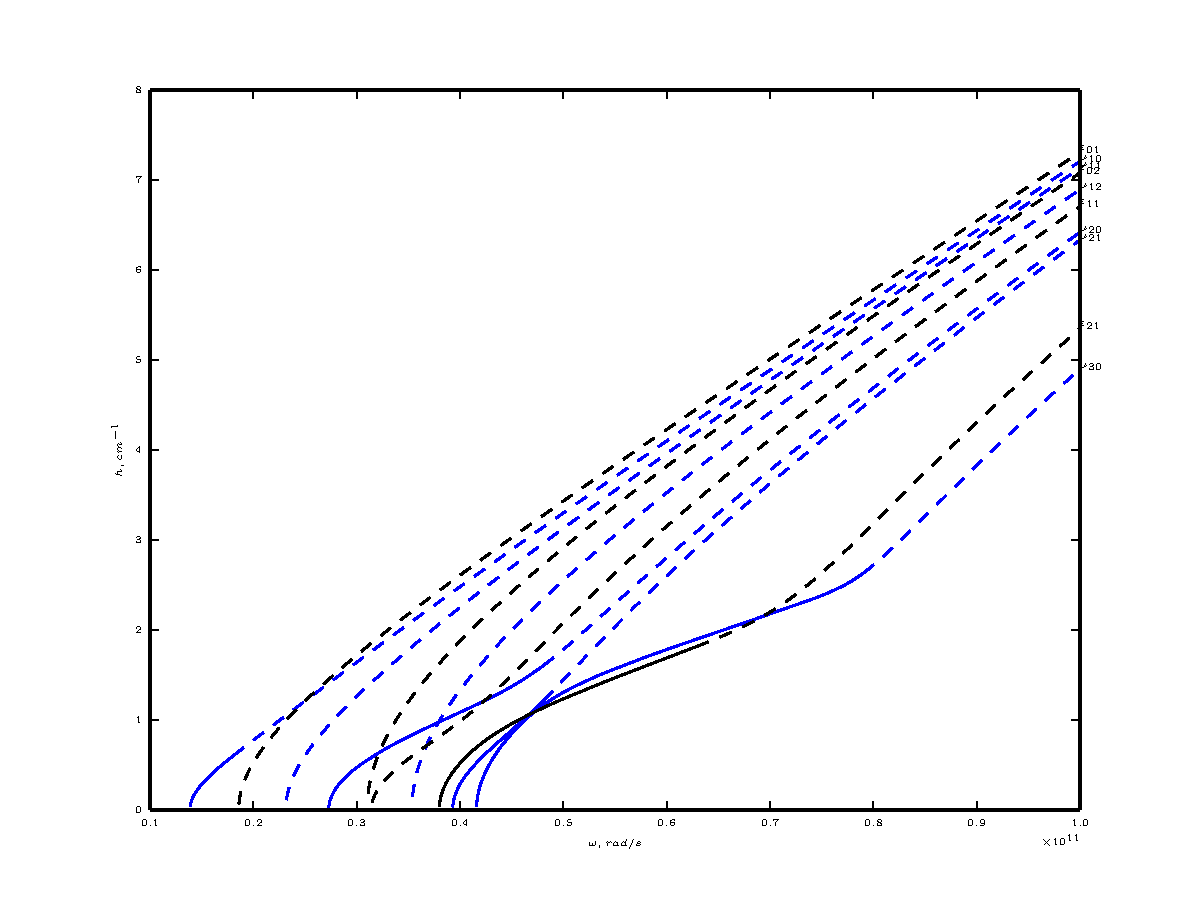
\includegraphics[width=.7\textwidth]{dispersion.pdf}
    \caption{Закон дисперсии для низших гармоник волновода}
    \label{fig:dispersion}
\end{figure}

